\documentclass[landscape]{article}

\usepackage[top=1.5cm, left = 1.5cm,right=1.5cm,bottom=1cm]{geometry}
\usepackage{tikz}

\newcommand{\cellheight}{18}
\pagestyle{empty}
\begin{document}

\centering
%Month \rule{3cm}{1pt}\\[1cm]

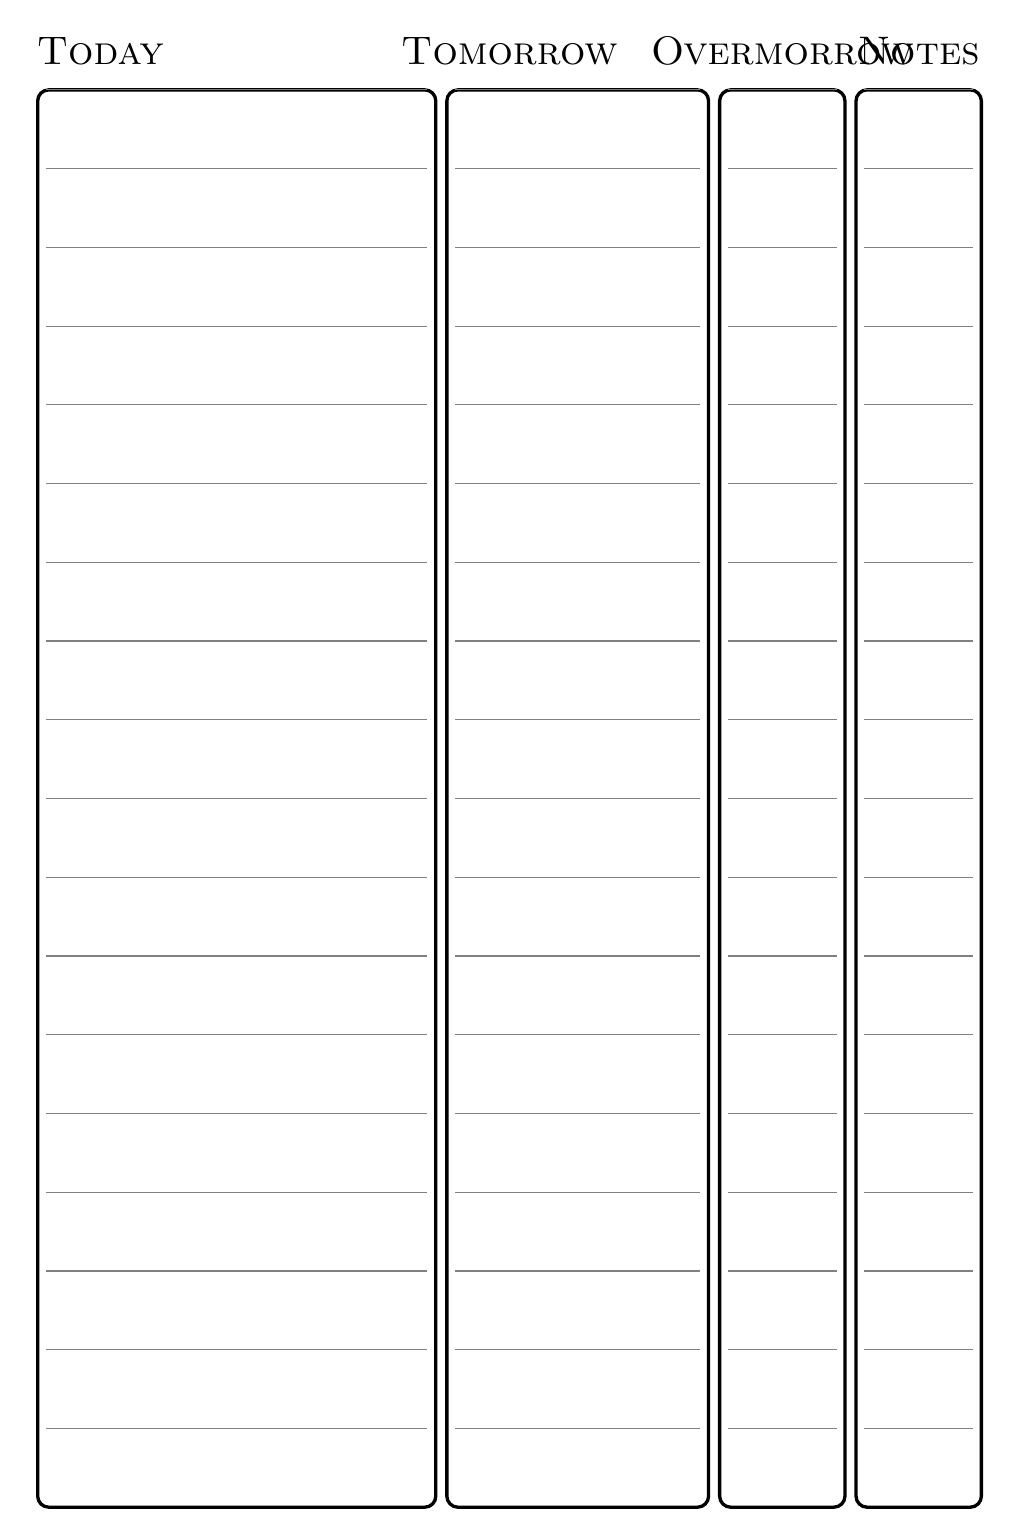
\begin{tikzpicture}

	
	\foreach \s/\D/\e in {0/Today/3,3/Tomorrow/5,5/Overmorrow/6 ,6/Notes/7}
	{	
		\node[] () at (\s*\linewidth/7+\linewidth/14,\cellheight+.5) {{\Large \sc \D}};
		\draw[rounded corners, very thick] (\s*\linewidth/7+.2em,0) rectangle (\e*\linewidth/7-.2em,\cellheight); 
		\foreach \y in {1,...,\cellheight}
		{
			\draw[gray] (\s*\linewidth/7+.5em,\y) -- (\e*\linewidth/7-.5em,\y);
		}
	}

\end{tikzpicture}


\end{document}